
\section{Introduction}
\ad{TODO talk about LLMs here, not BERT immediately} Pretrained language models (LLMs) \citep{devlin-etal-2019-bert} have achieved strong performance on text classification with a large amount of task-specific training data. However, in real world scenarios, collecting labeled data can be challenging due to expense and need for domain expertise.
%With the advent of powerful generalist models like GPT-4 \citep{Achiam2023GPT4TR}, LLaMa \citep{Touvron2023Llama2O}, Mistral \citep{jiang2023mistral} and Claude \citep{Bai2022TrainingAH}, zero-shot and few-shot prompting has become a common technique in solving multiple diverse tasks without parameter tuning. However, these models suffer from higher latency and are quite sensitive to prompts. 
Recently, several works have focused on generating texts using versatile LLMs such as GPT-4 \citep{Achiam2023GPT4TR}, Claude \citep{Bai2022TrainingAH}, Mistral \citep{jiang2023mistral}, Mixtal~\citep{jiang2024mixtral} and subsequently distill a student model on the synthetically generated data \citep{west-etal-2022-symbolic}. However, generated datasets suffer from a lack of diversity \citep{yu2023large} and regurgitate the biases of the teacher LLMs, which proliferate into the student model. Although prior works have utilized retrieval augmented generation for diverse dataset synthesis \citep{divekar2024synthesizrr}, here we focus on the more fundamental challenge of improving or controlling generations \emph{given a prompt and context}.


\begin{figure}[t!]
\centering
    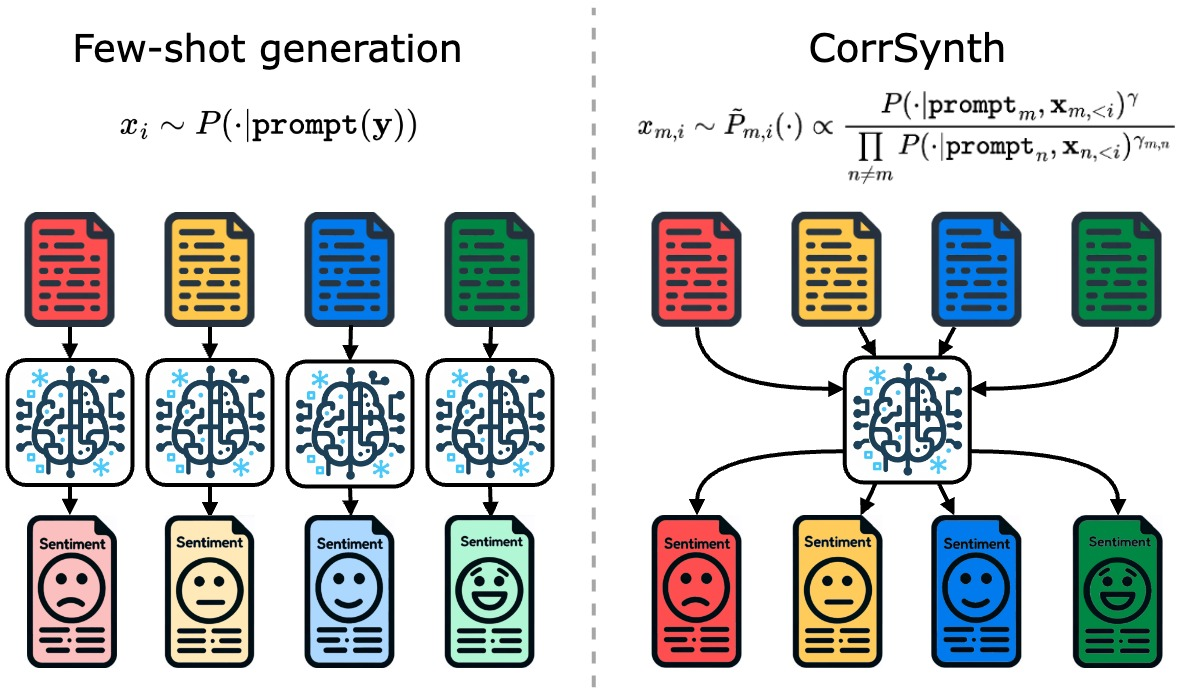
\includegraphics[width=0.95\linewidth]{figure/high-level-diagram-04-Oct-2024.jpg}
    \caption{\corrsyn\ introduces anti-correlation \mbox{between} examples, compared to few-shot generation.}
    \label{fig:corrsynth_high_level}
\vspace{-3ex}
\end{figure}

In particular, we focus on synthetic data generation for supervised text classification tasks and take the route of decoding time guidance based approaches \citep{sanchez2023stay,o2023contrastive,li2023contrastive,chuang2023dola}, which aim to tackle the challenge of improving diversity and faithfulness to target class in these generated datasets. Motivated by recent works on Classifier Free Guidance (CFG) \citep{sanchez2023stay}, we introduce a novel guidance based strategy, \corrsyn.\ad{State more clearly why we want to use CFG/guidance based approaches for dataset synthesis, and the problems of CFG (move that up here from later in the para).}
In \corrsyn{}, generations are kept faithful to the synthesis instruction, while introducing greater diversity and similarity to human text. \corrsyn{} is a correlated sampling approach which generates multiple sequences in parallel with strong inter-dependence between them. 
\ad{Too much }The main idea is as follows: when generating an instance of a particular class and sampling the next token, we \emph{contrast} its logits with logits corresponding to partially generated instances from other classes.
This is a simple but crucial change compared to CFG: in \corrsyn, the contrasting logits for a class/label are obtained from generations corresponding to other labels, whereas in CFG, the contrasting logits are obtained feeding back the generation for the current label into the LLM with prompts corresponding to other labels. To synthesize a $K$--class classification dataset, this requires $K$--times fewer forward passes compared to CFG. Furthermore, we can smoothly trade-off diversity and improve class-separability \ad{needs slightly more detail, seems to short}by introducing contrasts between logits from the same or different classes. 


% The main advantages of our approach over CFG are a) In a $K$-class classification setup, at the cost of $K$ forward passes, we get tokens for instances corresponding all the $K$ labels, whereas the natural extension of CFG to multi-class requires $K^2$ forward passes, and b) in CFG the effect of \emph{guidance} on later tokens is diminished due to the same generation being fed back into all the contrast terms\footnote{This diminishes the effect of the initial prompt on later generations} whereas in \corrsyn{} we use multiple generated sequences for contrast. \ad{Too much detail, move to method section, substantiate with Experimental results} 

In summary, our contributions are: \mbox{(1) we} develop a general correlated sampling approach, \corrsyn{}, that can generate multiple correlated sequences in parallel from an LLM, by explicitly introducing \textit{contrasts} between parallel generations during the sampling of each token, (2) we apply this to classification dataset synthesis, with the goal of improving diversity of synthetic generations, (3) we demonstrate how our method overcomes the limitations of CFG and controllable synthesis in regards to diversity and label-separation, (4) we benchmark our approach on tasks ranging from humor detection, sentiment analysis and topic classification in regional news headlines. Our intrinsic analysis find that \corrsyn{} generates datasets with higher representation of tail entities, lexical diversity and similarity to human text, and distillation accuracy of student models, compared to four state of the art baselines. 
